\documentclass[11pt, oneside]{article} 
\usepackage{geometry}
\geometry{letterpaper} 
\usepackage{graphicx}
	
\usepackage{amssymb}
\usepackage{amsmath}
\usepackage{parskip}
\usepackage{color}
\usepackage{hyperref}

\graphicspath{{/Users/telliott_admin/Tex/png/}}
% \begin{center} 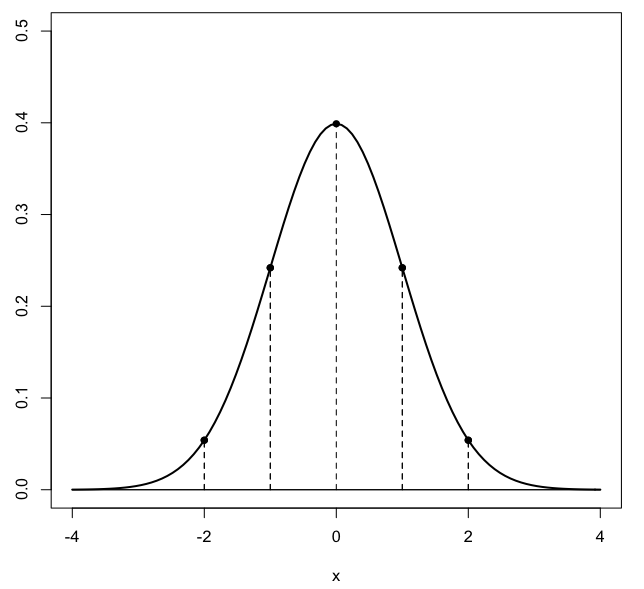
\includegraphics [scale=0.4] {gauss3.png} \end{center}

\title{Newton and the binomial}
\date{}

\begin{document}
\maketitle
\Large
The binomial can be viewed as a table of coefficients for the expansion of two terms (the binomial) raised to a power $n$:
\[ (a + b)^n = a^n b^0 + n a^{n-1} b^1 + \dots \]
\[ \ \ \ \ \ \dots+ n a^1b^{n-1} + a^0 b^{n} \]

The first few of these expansions are:
\[ (a+b)^1 = a + b \]
\[ (a+b)^2 = a^2 + 2ab + b^2 \]
\[ (a+b)^3 = a^3 + 3a^2b + 3ab^2 + b^3 \]
\[ (a+b)^4 = a^4 + 4a^3b + 6a^2b^2 + 4ab^3 + b^4 \]

In the case of $b = 1$ we obtain
\[ (1 + a)^1 = 1 + a \]
\[ (1 + a)^2 = 1 + 2a + a^2 \]
\[ (1 + a)^3 = 1 + 3a + 3a^2 + a^3 \]
\[ (1 + a)^4 = 1 + 4a + 6a^2 + 4a^3 + a^4 \]

Writing the coefficients with appropriate spacing, they can be viewed as a triangle (Pascal's Triangle).
\newpage 
\[ 1 \ \ 1 \]
\[ 1 \ \ 2 \ \ 1 \]
\[ 1 \ \ 3 \ \ 3 \ \ 1 \]
\[ 1 \ \ 4 \ \ 6 \ \ 4 \ \ 1 \]

One striking thing about the triangle is that each value which is not on an edge can be formed by adding together the two values that lie directly above it.  

One of its less well-known properties gives the Fibonacci numbers
\begin{center} 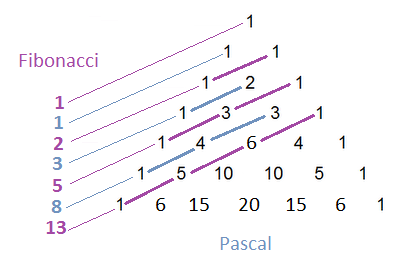
\includegraphics [scale=0.75] {pascalfib.png} \end{center}

If the coefficients are written in columns starting from the left (first version above), then each entry can be seen as the sum of the entry above it plus the one to the left and above, if it exists.

1 1

1 2 1

1 3 3 1

1 4 6 4 1

A general specification for the table is:
\[ (1 + a)^n = \sum_{k = 0}^n {{n}\choose{k}} a^{k} \] 
where as usual
\[ {{n}\choose{k}} = \frac{n!}{(n-k)! \ k!} \]
\[ = \frac{n \cdot (n-1) \cdot (n-2) \dots (n - k + 1)}{k!} \]

We used induction (\hyperref[sec:binomial_derivation]{\textbf{here}}) to prove this gives the correct coefficients for any value of the row $n$ and column $k$.

The standard table or triangle starts with $n = 1$, although we can easily extend it to $n = 0$.  That row is a single value of $1$.
\[ (a + b)^0 = 1 a^0 b^0 = 1 \] 

The table gives coefficients for the expansion with positive integers $n$.  The question we wish to answer here is:  what can be said about 
\[ (a + b)^{-2} \]
\[ (a + b)^{1/3} \]

\subsection*{Newton}

Newton wrote the binomial expansion in this way
\[ (P + PQ)^{m/n} \]
\[ = P^{m/n} + \frac{(m)}{(n)}P^{m/n}Q + \cdots \]
\[ + \frac{(m)}{(n)}\frac{(m-n)}{(2n)}P^{m/n}Q^2 + \cdots \]
\[ + \frac{(m)}{(n)}\frac{(m-n)}{(2n)}\frac{(m-2n)}{(3n)}P^{m/n}Q^3 + \cdots \] 

where the first three terms of an \emph{infinite series} are written on separate lines to emphasize the pattern connecting them.  The $k$th term, coefficients of $Q^k$, contains the coefficients of $Q^{k-1}$ times 
\[ \frac{(m-(k-1)n)}{(kn)} \]

This looks a little strange to modern eyes, but it's actually the same as the standard binomial, and it works for negative integers and fractional powers.

We can clean it up a little by factoring $P^{m/n}$ out of both sides
\[ (P + PQ)^{m/n} = P^{m/n}(1 + Q)^{m/n} \]
so that
\[ (1 + Q)^{m/n} = 1 + \frac{(m)}{(n)}Q + \cdots \]
\[ + (\frac{(m)}{(n)}) \frac{(m-n)}{(2n)}Q^2 + \cdots \]
\[  + \frac{(m)}{(n)}\frac{(m-n)}{(2n)}\frac{(m-2n)}{(3n)}Q^3 + \cdots \]

If we move $n$ into the numerator of the coefficients on the right hand side
\[ (1 + Q)^{m/n} = 1 + (m/n)Q + \cdots \]
\[ + (m/n)\frac{(m/n-1)}{2}Q^2 + \cdots \]
\[ + \ (m/n)\frac{(m/n-1)}{2}\frac{(m/n-2)}{3}Q^3 + \cdots \]

And now substitute $p = m/n$
\[ (1 + Q)^p = 1 + pQ + \cdots \]
\[ + \frac{p(p-1)}{2}Q^2 + \cdots \]
\[ +  \frac{p(p-1)}{2}\frac{(p-2)}{3}Q^3 + \cdots \]

Suddenly it looks familiar.  Newton's formula reduces to the standard binomial, but it has the additional feature that it allows the power to be fractional (and/or negative).  

Also, we don't write 
\[ {m/n}\choose{k} \]
or the factorial version, but still subtract $1,2,\cdots$ from $m/n$ for each successive cofactor.

\subsection*{usage}
The formula is (again)
\[ (1 + Q)^p = 1 + pQ + p\frac{(p-1)}{2}Q^2 + p\frac{(p-1)}{2}\frac{(p-2)}{3}Q^3 + \cdots \]

One way this is useful is to compute roots.  Let $p = 1/2$.  Then
\[ \sqrt{1 + x} = 1 + \frac{x}{2} - \frac{3}{16}x^2 + \frac{1}{16}x^3 + \dots \]

Another is to obtain a series for $1/(1+x)$.  Plug in $p = -1$ and the coefficients just alternate sign.
\[ (1+x)^{-1} = 1 - x + x^2 - x^3 + x^4 + \cdots  \]

Newton checked this by multiplying:
\[ 1 = (1+x)(1 - x + x^2 - x^3 + x^4 + \cdots)  \]
And if you know that the area under the curve is the logarithm, you can integrate the series for $1/(1+x)$ to obtain
\[ \ln(1+x) = x - \frac{x^2}{2} + \frac{x^3}{3} - \frac{x^4}{4} + \cdots \]
The logarithms obtained by this method can be easily verified.

\subsection*{derivation}
So far as I know Newton did not provide a proof of his version of the binomial theorem.  I found a discussion of how he came to it here:
\vspace{2 mm}

\url{http://www.quadrivium.info/MathInt/Notes/NewtonBinomial.pdf}

\begin{center} 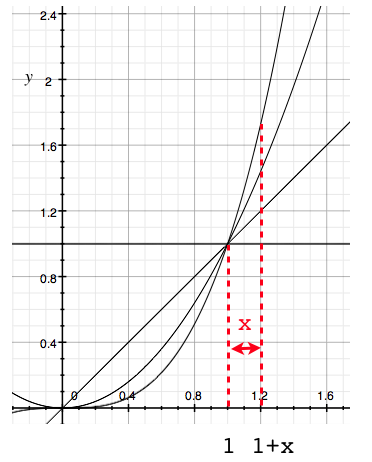
\includegraphics [scale=0.5] {newton1.png} \end{center}
Following Wallis, Newton studied expressions for the area under various curves.  Above: $y=x^n, n = \{0,1,2\}$.  These areas were apparently known, and I am not sure exactly how this was done, but I will use results obtained by integration.

It's perhaps a little confusing, but we will use $x$ here for two purposes.  First, the curves are $f(x)=x^n$. Second, we seek the area under each of these curves between the endpoints $1$ and $1+x$.  So for each $n$, we will compute the integral of $x^n - x^{n-1}$ and evaluate that between the limits $1$ and $1+x$.
\vspace{2 mm}

\noindent For $y = x^0$, the area under the curve is just $x$.
\vspace{2 mm}

\noindent For $y = x^1$, the \emph{additional} area is $(1/2)x^2$.  
\vspace{2 mm}

\noindent For $y = x^2$ we have that the additional area is
\[ A = \int_1^{1+x} x^2 - x \ dx =  \frac{1}{3} x^3 - \frac{1}{2} x^2 \ \bigg |_1^{1+x} \]
\[ = \frac{1}{3} (1+x)^3 - \frac{1}{3}(1) - \frac{1}{2} (1+x)^2 - \frac{1}{2}(1) \]
\[ = \frac{1}{3} (1 + 3x + 3x^2 + x^3) - \frac{1}{3}(1) - \frac{1}{2} (1 + 2x + x^2) - \frac{1}{2}(1) \]
\[ = x + x^2 + \frac{1}{3}x^3 - x - \frac{1}{2}x^2 \]
\[ = \frac{1}{2}x^2 + \frac{1}{3}x^3 \]
Hence the total area is
\[ A_{tot} = x + x^2 + \frac{1}{3}x^3 \]
\noindent For $y = x^3$ we have that the additional area is
\[ A = \int_1^{1+x} x^3 - x^2 \ dx =  \frac{1}{4} x^4 - \frac{1}{3} x^3 \ \bigg |_1^{1+x} \]
\[ = \frac{1}{4} (1+x)^4 - \frac{1}{4}(1) - \frac{1}{3} (1+x)^3  - \frac{1}{3}(1)\]
\[ = \frac{1}{4}(4x + 6x^2 + 4x^3 + x^4) - \frac{1}{3} (3x + 3x^2 + x^3) \]
\[ = \frac{1}{2}x^2 + \frac{2}{3}x^3 + \frac{1}{4}x^4 \]
Hence the total area is
\[ A_{tot} = x + \frac{3}{2}x^2 + \frac{3}{3}x^3 + \frac{1}{4}x^4 \]
If we carried out this exercise for the fourth and fifth powers we would find
\[ A_{tot} = x + \frac{4}{2}x^2 + \frac{6}{3}x^3 + \frac{6}{4}x^4 + \frac{1}{5}x^5 \]
\[ A_{tot} = x + \frac{5}{2}x^2 + \frac{10}{3}x^3 + \frac{10}{4}x^4 + \frac{5}{5}x^5 + \frac{1}{6}x^6 \]
\vspace{2 mm}

If we look carefully at what we've obtained, we see that there is a sum of terms like $x^p/p$ times a cofactor which goes like Pascal's triangle or a standard binomial expansion (and indeed, that's where it came from).  Newton organized the cofactors into a table.
\[
\begin{matrix}
\text{p}  \\
x/1  \\
x^2/2 \\
x^3/3 \\
x^4/4 \\
x^5/5 \\
x^6/6 \\
x^7/7
\end{matrix} \ \ \ \
\begin{matrix}
0 & 1 & 2 & 3 & 4 & 5  \\
1 & 1 & 1 & 1 & 1 & 1  \\
0 & 1 & 2 & 3 & 4 & 5 \\
0 & 0 & 1 & 3 & 6 & 10 \\
0 & 0 & 0 & 1 & 4 & 10 \\
0 & 0 & 0 & 0 & 1 & 5 \\
0 & 0 & 0 & 0 & 0 & 1 \\
0 & 0 & 0 & 0 & 0 & 0
\end{matrix}
\]


That is, we have for $x^2$ that the area is
\[ (1)x + (2)\frac{1}{2}x^2 + (1)\frac{1}{3}x^3 = x + x^2 + \frac{1}{3}x^3 \]

Newton noticed the pattern which is so clear in Pascal's triangle, that the coefficients can be generated by addition.  For example, the $6$ in the column for $n=4$ is generated by adding together the two entries of $3$ to its immediate left and upper-left.  Thus, having the first row (all $1$), and the column under $n=0$, one can generate the rest of the table mechanically.

Now, Newton says, what happens if we add an additional column for $n=-1$, and it follows the rule that the entry in the first row must be $1$?
\[
\begin{matrix}
\text{p}  \\
x/1  \\
x^2/2 \\
x^3/3 \\
x^4/4 \\
x^5/5 \\
x^6/6 \\
x^7/7
\end{matrix} \ \ \ \
\begin{matrix}
-1 & 0 & 1 & 2 & 3 & 4 & 5  \\
\ \ 1 & 1 & 1 & 1 & 1 & 1 & 1  \\
\ \ . & 0 & 1 & 2 & 3 & 4 & 5 \\
\ \ . & 0 & 0 & 1 & 3 & 6 & 10 \\
\ \ . & 0 & 0 & 0 & 1 & 4 & 10 \\
\ \ . & 0 & 0 & 0 & 0 & 1 & 5 \\
\ \ . & 0 & 0 & 0 & 0 & 0 & 1 \\
\ \ . & 0 & 0 & 0 & 0 & 0 & 0
\end{matrix}
\]
How do we fill  in the missing entries?  By using the addition rule!  The first missing value must be a $-1$, so that it plus the $1$ above add together to give the $0$ to its right.
\[
\begin{matrix}
\text{p}  \\
x/1  \\
x^2/2 \\
x^3/3 \\
x^4/4 \\
x^5/5 \\
x^6/6 \\
x^7/7
\end{matrix} \ \ \ \
\begin{matrix}
-1 & 0 & 1 & 2 & 3 & 4 & 5  \\
\ \ 1 & 1 & 1 & 1 & 1 & 1 & 1  \\
-1 & 0 & 1 & 2 & 3 & 4 & 5 \\
\ \ . & 0 & 0 & 1 & 3 & 6 & 10 \\
\ \ . & 0 & 0 & 0 & 1 & 4 & 10 \\
\ \ . & 0 & 0 & 0 & 0 & 1 & 5 \\
\ \ . & 0 & 0 & 0 & 0 & 0 & 1 \\
\ \ . & 0 & 0 & 0 & 0 & 0 & 0
\end{matrix}
\]
He filled out the rest of the column for $n=-1$ using this idea.  
\[
\begin{matrix}
\text{p}  \\
x/1  \\
x^2/2 \\
x^3/3 \\
x^4/4 \\
x^5/5 \\
x^6/6 \\
x^7/7
\end{matrix} \ \ \ \
\begin{matrix}
-1 & 0 & 1 & 2 & 3 & 4 & 5  \\
\ \ 1 & 1 & 1 & 1 & 1 & 1 & 1  \\
-1 & 0 & 1 & 2 & 3 & 4 & 5 \\
\ \ 1 & 0 & 0 & 1 & 3 & 6 & 10 \\
-1 & 0 & 0 & 0 & 1 & 4 & 10 \\
\ \ 1 & 0 & 0 & 0 & 0 & 1 & 5 \\
-1 & 0 & 0 & 0 & 0 & 0 & 1 \\
\ \ 1 & 0 & 0 & 0 & 0 & 0 & 0
\end{matrix}
\]
This gives the series for $1/(1+x)$ that we have above.  
\[ \frac{1}{1+x} = 1 - x + x^2 - x^3 + x^4 + \cdots  \]

Using this idea, one can fill in the table for the negative integers.  What about fractional powers?
\[
\begin{matrix}
\text{p}  \vspace{2 mm} \\
x/1  \\
x^2/2 \\
x^3/3 \\
x^4/4 \\
x^5/5 \\
x^6/6
\end{matrix} \ \ \ \
\begin{matrix}
-1 & -\frac{1}{2} & 0& \frac{1}{2} & 1& \frac{3}{2}  & 2 & \frac{5}{2}  & 3   \vspace{2 mm}  \\
\ \ 1 & \ \ 1 & 1 & 1 & 1 & 1 & 1 & 1 & 1 \\
-1 & \ \ . & 0 & . & 1 & . & 2 & . & 3 \\
\ \ 1 & \ \ . & 0 & . & 0 & . & 1 & . & 3 \\
-1 &  \ \ .  & 0 & . & 0 & . & 0 & . & 1 \\
\ \ 1 &  \ \ . & 0 & . & 0 & . & 0 & . & 0 \\
-1 &   \ \  . & 0 & . & 0 & . & 0 & . & 0 \\
\end{matrix}
\]
After a lot of work, Newton comes to two simple ideas.  First, the addition rule remains in place, for entries that are separated by a whole unit.

The missing entries in the table above depend not on the entries to the immediate left, but one more column over.  Given one of these missing entries, the entire row can be filled in.  Let's try
\[
\begin{matrix}
\text{p}  \vspace{2 mm} \\
x/1  \\
x^2/2 \\
x^3/3 \\
x^4/4 \\
x^5/5
\end{matrix} \ \ \ \
\begin{matrix}
-1 & -\frac{1}{2} & 0& \ \ \frac{1}{2} & 1& \frac{3}{2}  & 2 & \frac{5}{2}  & 3   \vspace{2 mm}  \\
\ \ 1 & \ \ 1 & 1 & \ \ 1 & 1 & 1 & 1 & 1 & 1 \\
-1 & \ \ -1/2 \ \ & 0 & \ \ 1/2 & 1 & 3/2 & 2 & 5/2 & 3 \\
\ \ 1 & \ \ . & 0 &  . & 0 & . & 1 & . & 3 \\
-1 &  \ \ .  & 0 & . & 0 & . & 0 & . & 1 \\
\ \ 1 &  \ \ . & 0 & . & 0 & . & 0 & . & 0 \\
\end{matrix}
\]
I won't fill in the rest of the entries, except the column for the $1/2$ power
\[
\begin{matrix}
\text{p}  \vspace{2 mm} \\
x/1  \\
x^2/2 \\
x^3/3 \\
x^4/4 \\
x^5/5
\end{matrix} \ \ \ \
\begin{matrix}
-1 & -\frac{1}{2} & 0& \ \ \frac{1}{2} & 1& \frac{3}{2}  & 2 & \frac{5}{2}  & 3   \vspace{2 mm}  \\
\ \ 1 & \ \ 1 & 1 & \ \ 1 & 1 & 1 & 1 & 1 & 1 \\
-1 & \ \ -1/2 \ \ & 0 & \ \ 1/2 & 1 & 3/2 & 2 & 5/2 & 3 \\
\ \ 1 & \ \ . & 0 &  -1/4 & 0 & . & 1 & . & 3 \\
-1 &  \ \ .  & 0 & \ \ 3/16 & 0 & . & 0 & . & 1 \\
\ \ 1 &  \ \ . & 0 & -15/96 & 0 & . & 0 & . & 0 \\
\end{matrix}
\]

\subsection*{Computation of $\pi$}
The series generated under the $1/2$ power is 
\[ x - \frac{1}{4} \ \frac{x^2}{2} + \frac{3}{16} \ \frac{x^3}{3} - \frac{15}{96} \ \frac{x^4}{4}  + \cdots \]
if $x = \sqrt{1-u^2}$, this is

\[ x - \frac{1}{4} \ \frac{x^2}{2} + \frac{3}{16} \ \frac{x^3}{3} - \frac{15}{96} \ \frac{x^4}{4}  + \cdots \]
is the area under the quarter-circle ($\pi/4$), when $x=1$.
\[ \frac{\pi}{4} = 1 - \frac{1}{4} \ \frac{1}{2} + \frac{3}{16} \ \frac{1}{3} - \frac{15}{96} \ \frac{1}{4}  \]
\[ = 1 - \frac{1}{8} + \frac{3}{48} - \frac{15}{384} + \cdots  \]

\end{document}  